\documentclass{article}[a4]
\usepackage{url}
\usepackage{epcc}
\usepackage{graphicx}
\usepackage[nottoc,numbib]{tocbibind}

\begin{document}
\title{Project Preparation Report}
\author{Jim Walker}
\date{\today}

\makeEPCCtitle

\thispagestyle{empty}

\pagebreak
\tableofcontents
\pagebreak

\section{Introduction}
This Project Preparation report first provides a review of previous dissertations. It then presents the necessary background and literature for the project, and details a project proposal. A workplan for the project is sketched out, wherein we present chapter summaries and headings for the final dissertation alongside a Gantt chart. We identify risks and provide mitigations for them, before explaining our preliminary findings.
\section{Dissertation Review}
The two dissertations I have chosen to review are \textit{Assessing the Performance of Optimised Primality Tests}~\cite{Curry2016} by Cameron Curry, and \textit{Extending ePython to support ePython interpreting across multiple interconnected Epiphany processors}~\cite{Liang2017} by Dongyu Liang. I have chosen these dissertations because they are relevant to my own project. Liang's \textit{Extending ePython} is focused on a programming language that is not typical in the HPC space, just my project will. Curry's \textit{Optimised Primality Tests} compared implementations of a core HPC function. My project will compare my Rust implementation of some HPC code, with its original C implementation. In this review, I will summarise both dissertations, and then discuss what features of the dissertation I should emulate or avoid.

\subsection{Extending ePython}

Liang's \textit{Extending ePython} chiefly aims to extend ePython, a python interpreter for the Epiphany processor, to `support parallel programming on multiple interconnected Epiphanies'~\cite{Liang2017}. An Epiphany processor has 16 cores, or e-cores, which makes it a useful platform for highly parallel codes. Liang first presents the technologies and paradigms which will they will use in their work. They go on to briefly describe the construction of their Epiphany cluster, before discussing at length their non trivial extension of ePython. Lastly, Liang closes with a results section which proves his achievements.

 \textit{Extending ePython} shows that Liang has made a useful contribution to the territory. Their technical achievement in extending ePython's parallelism to cover many nodes is notable, especially as Liang claims to make this change without compromising or altering the ePython programmer's interface. However, we can unfortunately only take his word for this, as his appendices only provide his modified ePython. Liang does not include a listing of the form the original ePython would have taken.

 The introduction of \textit{Extending ePython} contains the assertion by Liang that the Epiphany processor `is  notoriously  difficult  to  program'. Liang does not cite any sources for this claim, which is made somewhat dubious by the existance of a Python implementation precisly for the Ephipany processor.

 In the General Methodologies section (3.1.2) of the Construction (3.1), Liang discusses  `The principle of modifying ePython in the whole project is to make as few unnecessary adaptations as possible'. Liang goes on to describe the methodologies used to develop their extensions, and clearly prioritises and justifies their design decisions. Unfortunately, in this section Liang goes on to  discuss their implementation of host and device side activities. Whilst these details are useful to the reader in understanding how the e-cores communicate with each other, their inclusion in this section detracts from its clarity. This section could potentially be improved by moving the discussion of host and divice side activities into their own part of the dissertation.

 Sections 3.2 and 3.3 of \textit{Extending ePython} contain a methodical presentation of Liang's extensions. Liang include all the detail necessary to understand what these extensions consist of, and provides useful figures to help the reader visualise some concepts. As these are very techical sections, it could perhaps be improved by the additions of some listings of psuedo-code to clarify the author's occasionally verbose description of a complex technology.

 We also question Liang's claims on the stability of their extension to ePython. Firstly, they do not precisly define what they mean by stability, if they means their system is numerically stable or if it simply does not crash. Secondly, Liang presents their code running on 32 cores across two nodes, presumbly because they only had access to two nodes. Liang goes on to make the claim that their extension `could have become a cornerstone of the Supercomputer.io project'~\cite{Liang2017}, and saved it from its early end. The Supercomputer.io project was an attempt to collect multiple volunter ephiphany based nodes across the internet to build an extremely large, extremely distributed cluster. Whilst Liang's extension to ePython would certainly have been a valuable contribution to the problems faced by Supercomputer.io, it is somewhat spurious for them to claim that their work could have been a `cornerstone' for this project. The high latency and large scale of the Supercomputer.io project is not really comparable to running a small cluster of two nodes, connected through a LAN.

 Liang closes with some benchmarks to display the performance of their ePython extensions. Liang's range of tests is comprehensive, and figure 4.5, showing the good parallel efficiency of the implementation is particularly intersting. We feel that figure 4.4, which shows the results of the strong scaling test on the cluster, could be improved by using more, larger problem sizes, and plotting them against speedup. This change would help make the test more indicative of future use cases, and make change in performance size and its affect on performance starker.

\subsection{Optimised Primality Tests}

In \textit{Optimised Primality Tests} Curry seeks to compare three different implementations of the Fermat Tests, to assess which one PrimeGrid, a large distributed HPC project, should use. He argues that this is an important problem due to the use of extensive use of primes in computing, particularly cryptography. Curry also hopes to modify the Genefer implementation of the Fermat Test so that its residue calculation is consistent with other Fermat Test implementations.

Curry goes into great detail on the theoretical and practical background to his work. His frequent use of equations in section 2.1.4, `GFN Primes \& The Discrete Weighted Transform', show a firm grasp of the mathematical nature of his work, and how it is effected in harderware. Unfortunately Curry fails to emphasise how this background relates to his performance tests.  Whilst he does account for the `practicalities of digit representation in hardware', he does not make clear what he's doing effect this will have on his work, or how it is relavent to the specific performances of the implementations of the fermat tests.

Curry goes on to describe his performance testing  methodology, introducing the well accepted Roofline Model~\cite{williams2009}\cite{hennessy2011computer}\cite{asanovic2009view}, which he uses to find the peak perofrmance ofthe processors he will run his test on. This valuable section is well documented and supported by useful figures and brief commands. Curry simultaneously justifies his choices whilst detailing them with the necessary clarity to make his testing reproducible.

Curry finds Genefer to be the faster than both the LLR and OpenPFGW's Fermat Test implementations and thoroughly investigates why that is, using tools such as CrayPAT and the afore-mentioned RoofLine model to identify potential hardware bottlenecks or sources of softare overhead. That Curry goes so far as to create a micro benchmark to test an assumption shows a rigourus approach to his experimentation.

Curry is motivated to modify Genefer's residue calculation due to it's lack of consistency with OpenPFGW and LLR. This difference `is not an indication of incorrect results, it is simply a different representation of the least significant 64 bits'. He goes onto document his modification of Genefer's residue calculation, first implementing it with the same library used by OpenPFGW and LLR and then developing his own implementation of it to maintain the application's portability. Whilst Curry's implementation of a consistent residue for Genefer is shown to be correct, Curry is correct to call this feature only 'potentially production ready for use', as he only shows us a few comparisons between calculations. To be sure that this implementation was ready would require much more testing of it than has been carried out here.

\section{Background and Literature Review} %Why
Programming was once incredibly hard. The very first electronic computers were programmed in hexadecimal by people intimately familiar with their machines. These programs were brittle and often illegible to anyone but the author. However, when compilers were introduced it was argued by some that compilers produced machine code that was slow and not as precise as continuing to write in hexadecimal~\cite{Jargon}.

Technology has vastly improved since the first compilers were written, and so too has the ease and accessibility of programming. These days programming in Python, one of the most accessible languages, is taught to secondary school children, who require little to no knowledge of the machine they are programming on.

\begin{table}[h]

  \centering
  \label{tab:langs}
  \begin{tabular}{|c|c|c|c|c|}
    \hline
    & \textbf{HECToR Phase 2a} & \textbf{HECToR Phase 2b} & \textbf{HECToR Phase 3} & \textbf{Archer} \\
    \hline
    Fortran & 66.3\% & 65.2\% & 66.8\% & 69.3\% \\
    \hline
    C++ & 8.9\% & 2.7\% & 4.4\% & 7.4\% \\
    \hline
    C & 0.4\% & 3.6\% & 5.4\% & 6.3\% \\
    \hline
    Unidentified & 29.1\% &  30.0\% & 24.2\% & 19.4\% \\
    \hline
  \end{tabular}
  \caption{Programming Language Usage on some HPC Machines~\cite{Turner2015}}
\end{table}

High Performance Computing (HPC) is often seen to be lagging behind these language advances. Programming large, extremely fast programs to run on many cores on many nodes is still hard. Whilst these programs are now less brittle and are easier to read, they are still difficult to program to a high standard. This difficulty arises in part because the two most common languages in HPC, C and FORTRAN, (see table~\ref{tab:langs}) are not memory safe. Consider the program in the listing below, which shows how a programmer might lose track of which thread is writing to which value at which time.

\begin{figure}
  \centering
  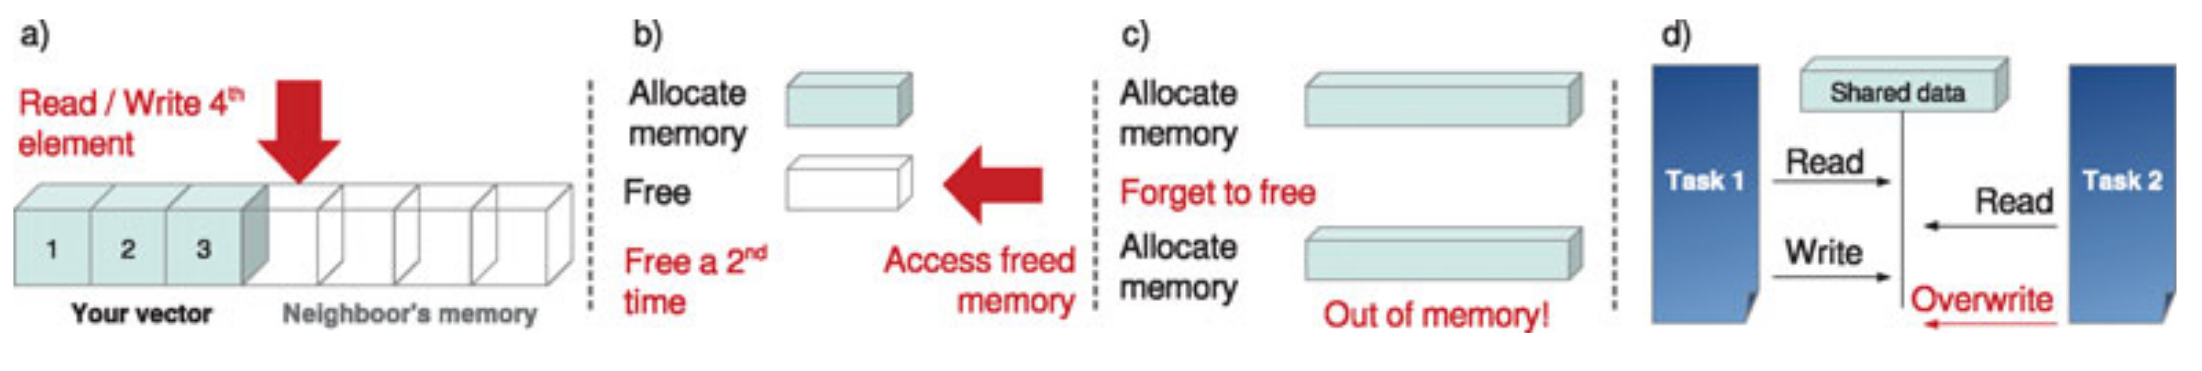
\includegraphics[width=\linewidth]{figures/memory-safety.png}
  \caption{Potential Memory Safety Related Bugs~\cite{blanco-cuaresma_bolmont_2016}}
  \label{fig:mem}
\end{figure}

Until now, languages which can offer memory safety, or other useful types of safety such as type safety, have been thought to be unsuitable for HPC due to the speed cost of using them. The Rust programming language has began to challange this paradigm.

Rust is a programming language, released in 2014 that uses an ownership model of memory to offer strong safety guarantees. `[P]ure Rust programs are guaranteed to be free of memory errors (dangling pointers, doublefrees) as well as data races'~\cite{Matsakis:2014}. Alongside this, Rust's lack of a garbage collector and fine grained memory control allow the language to achieve speeds comparable to C and FORTRAN. These features of Rust make it a plausible contender to become an accepted HPC language.

Some work has been done to investigate the applicability of Rust in scientific programming for bio-informatics~\cite{bioinformatics} and astro-physics~\cite{blanco-cuaresma_bolmont_2016}. Scientific kernels and apps such as the ones featured in these papers are common in HPC. The results of these investigations have been promising, and show that Rust is as fast, if not faster than implementations written in C or FORTRAN.

\section{Project Proposal} % What
Port a HPC mini app or benchmark into Rust. Document process and learning curve. Compare performance. Go into technical detail about how it works like it does.

Mini app criteria, longlist, how will i shortlist or choose from this
\subsection{Project Goals}
\begin{itemize}
  \item Find a software artifact that is representative of HPC use
  \item Port that software artifact to Rust
  \item Assess how easily C/++ developers can understand Rust
  \item Find theoretical hardware capabilities
  \item Single Node Performance Tests
  \item Strech goal - Multi node performance test
\end{itemize}
\section{Workplan} % How
\begin{itemize}
  \item Select benchmark/mini app to port
  \item Develop Mini App
\end{itemize}

Work item - thing that you get
Stretch goal - Rust MPI
\begin{description}
  \item[Introduction]:
  \begin{itemize}
    \item Current state of Programming Languages in HPC
    \item How are benchmarks/miniapps used in HPC
  \end{itemize}
  \item[Background]:
    \begin{itemize}
    \item What do programming languages need to be used in HPC?
    \item Why did D fail to replace C/++ in HPC? What does this mean for Rust?
    \item What is Rust? What are its unique features of interest?
    \item How will my dissertation provide an indication of Rust's ability to succeed in HPC?
  \end{itemize}
  \item[Implementation]:
  \begin{itemize}
    \item Overview of Software which I will port
    \item Technical description of my implementation
    \item Discussion of what implementation and learning Rust was like
  \end{itemize}
  \item[Performance Analysis]:
  \begin{itemize}
    \item How does performance compare to original app?
    \item How close do we get to hardware limit?
    \item How are both implementations affected by scaling?
  \end{itemize}
  \item[Conclusion] :
  \begin{itemize}
    \item Summary of findings
    \item Further work
  \end{itemize}
\end{description}

Gantt Chart to go here

\section{Risk Analysis}
We present our risk register.
\begin{table}[h]
  \centering
  \begin{tabular}{p{4cm} c c p{4cm}}
    Risk & Probability & Severity & Mitigation \\
    \hline
    Poor port selection & Medium & Medium & Confirm selection with advisers \\ \hline

    No knowledge of Rust amongst EPCC staff & High & Low & Rely on Rust community for language issues \\
    \end{tabular}
  \caption{Risk Register}
  \label{tab:risk}
\end{table}
\section{Preliminary Findings}
Rust is capable of very aggressive optimisation. It is being used more and more frequently. Parallel iterator from the rayon crate is comparable to OpenMP.

Rust has been installed on Cirrus
\section{Conclusion}
\pagebreak
\bibliographystyle{plain}
\bibliography{bib}
\end{document}
